%%%%%%%%%%%%%%%%%%%%%%%%%%%%%%%%%%%%%%%%%%%%%%%%%%%%%%%%%%%%%%%%%%%%%%%%
% Preamble
%%%%%%%%%%%%%%%%%%%%%%%%%%%%%%%%%%%%%%%%%%%%%%%%%%%%%%%%%%%%%%%%%%%%%%%%
\documentclass[11pt]{article}
%
% Packages and other includes
% Pagination
\usepackage[letterpaper, margin=1in]{geometry}
\usepackage{emptypage}
\usepackage[backend=biber,style=chem-acs]{biblatex}
\addbibresource{references.bib}
\usepackage{ulem}
\usepackage{xcolor}
\usepackage{mhchem}
%
% Fonts
\usepackage[T1]{fontenc} % best for Western European languages
\usepackage{lmodern} % Latin Modern instead of CM
\usepackage{textcomp} % required to get special symbols
%
% Math
\usepackage{amsmath, amssymb}
\usepackage{braket}
%
% Graphics, floats, tables
\usepackage{graphicx, color, float, array}
%
% Hyperlinks
\usepackage{hyperref}
%
%
% Definitions and settings
% Paragraph indent and spacing
\setlength{\parskip}{0.4\baselineskip}
\setlength{\parindent}{0in}
%
%
% Title, authors, date
\title{\textbf{Worksheet 6}}
\date{\vspace{-2em}February 8th, 2022}
%
%
%%%%%%%%%%%%%%%%%%%%%%%%%%%%%%%%%%%%%%%%%%%%%%%%%%%%%%%%%%%%%%%%%%%%%%%%
% Main document
%%%%%%%%%%%%%%%%%%%%%%%%%%%%%%%%%%%%%%%%%%%%%%%%%%%%%%%%%%%%%%%%%%%%%%%%
%

\begin{document}

\maketitle

Collaborations are encouraged and students must report all collaborators
on each assignment. All external sources (websites, books) must be
cited. An \textit{extra credit} (\textit{EC}) problem will be available per
assignment. Please submit a completed homework on-time to receive \textit{EC}
and no partial \textit{EC} (all parts must be correct) will be given out.
Additional problems are listed at the end of each assignment. This week's
assignment is due \textit{Tuesday, Feb 15th at 10:00am.}

1. (5 pts) \textbf{Direct Carbon Fuel Cell.} This technology uses a carbon rich
material and converts the chemical energy in solid carbon to eletricity through
fuel cell reactions and electrochemical oxidation. It has the following reactions

  Anode: C(s) + 2 O$^-$(g) $\rightarrow$ CO$_2$(g) + 4 e$^-$

  Cathode: 4 e$^-$ + O$_2$(g) $\rightarrow$ 2 O$^-$(g)

\begin{figure}[hbpt]
  \centering
  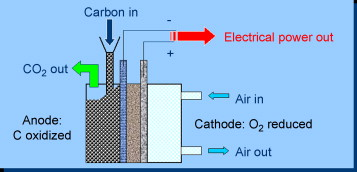
\includegraphics[scale=1]{direct_carbon.jpg}
  \caption{Illustration of direct carbon fuel cell}
\end{figure}
Report all values to 3 significant digits.

(a) What is the overall reaction?

(b) The standard enthalpy ($\Delta H^\circ$) and standard Gibbs
free energy ($\Delta G^\circ$) are $-393.5$ kJ/mol and $-394.5$ kJ/mol,
respectively. What is the entropy change?

(c) Assuming $100\%$ efficiency, how much carbon (in kg) is needed to deliver
1 MWh of electricity?

\pagebreak

2. (2 pts) \textbf{Temperature dependence of $K$.} ATP is a compound that provides energy
for biochemical reactions in the body when it undergoes hydrolysis. For the hydrolysis
of ATP at $37^\circ\text{C}$ (normal body temperature) $\Delta H^\circ_r = -20.$ and
$\Delta S_r^\circ = +34 \text{J}\cdot\text{K/mol}$. Assuming that these quantities are independent
of temperature, calculate the temperature at which the equilibrium constant for the
hydrolysis of ATP becomes greater than 1. Report to 2 significant figures.

% Atkins 10.114

\vspace{2in}

3. (4 pts) \textbf{Mixing Ideal Gases.} A container is divided into two equal compartments.
One contains 3.0 mol CO$_2$ and the other contains 1.0 mol N$_2$ at $25^\circ\text{C}$.
Assume ideal gas behavior. Calculate the Gibbs free energy of mixing when the partition
is removed. Report to 2 significant figures.

% http://people.se.cmich.edu/teckl1mm/pchemi/chm351ch7bf01.htm

\vspace{2in}

4. (4 pts) \textbf{No Laughing Matter.} Nitrous oxide (N$_2$O), known as laughing gas,
has been the largest ozone-depleting substance and has a lifetime of 114 years in the
atmosphere. N$_2$O undergoes a series of reactions:
\begin{center}
  \makebox[4in]{N$_2$O(g) + O(g) + $h\nu$ $\rightarrow$ 2 NO(g) \hspace{1in}} (1)\par
  \makebox[4in]{\ce{NO(g) + O$_3$(g) <=> NO$_2$(g) + O$_2$(g)}$\,\,$ $K = 7\times 10^{103}$} (2)\par
  \makebox[4in]{\ce{NO$_2$(g) + O(g) <=> NO(g) + O$_2$(g)}$\,\,$ $K = 5.8\times 10^{-34}$} (3)\par
\end{center}
Based on the reactions, describe in words how N$_2$O is impacting ozone concentration.
\textit{Hint:} Look at the overall reactions (2) and (3). What role does NO and NO$_2$ play?

\pagebreak

\textbf{Ozone Depletion}

5. (6 pts) \textit{Extra Credit:} Reactions between gases in the atmosphere are not at equilibrium,
but for a thorough understanding of them we need to study both the rates at which they take
place and their behavior under equilibrium conditions.

(a) Depletion of ozone (O$_3$(g)) in the stratosphere can be summarized by:
\begin{center}
  \ce{2 O$_3$(g) <=> 3 O$_2$(g)}
\end{center}
Determine the standard Gibbs free energy, standard enthalpy and standard entropy for the
reaction.

(b) In part (a), what is the equilibrium constant of the reaction at $25^\circ\text{C}$?
What is the significance of your answer with regard to ozone depletion?

(c) At any given time, ozone molecules are constantly formed and destroyed. One
of the reactions that depletes ozone is:
\begin{center}
  \ce{O$_3$(g) + O(g) <=> 2 O$_2$(g)}
\end{center}
Calculate the value of the equilibrium constant for this reaction at $25^\circ\text{C}$
given that at that temperature the reaction is catalyzed by NO$_2$ molecules in a two-step
process:
\begin{center}
  \ce{NO$_2$(g) + O(g) <=> NO(g) + O$_2$(g) $\,\,$ $K = 7\times 10^{103}$} \\
  \ce{NO(g) + O$_3$(g) <=> NO$_2$(g) + O$_2$(g) $\,\,$ $K = 5.8\times 10^{-34}$}
\end{center}

(d) Determine the standard Gibbs free energy of formation of oxygen atoms from part (c).

(e) The Van't Hoff equation describes the equilibrium constant $K$ in term of temperature
$T$, gas constant $R$, standard enthalpy ($\Delta H^\circ$) and standard entropy
($\Delta S^\circ$):
\begin{equation}
  \ln K = -\frac{\Delta H^\circ}{RT} + \frac{\Delta S^\circ}{R}
\end{equation}
For the reaction \ce{N$_2$(g) + O$_2$(g) <=> 2 NO(g)}, will this reaction proceed further
at very low temperatures of the stratosphere or high temperatures in an internal combustion
engine? What implications do this suggest?

(f) An equimolar mixture of N$_2$(g) and O$_2$(g) with a total pressure of 4.00 bar
was allowed to come to equilibrium in the reaction in part (e) at 1200. K. What will
be the partial pressure of each reactant and product at equilibrium?

% Atkins 10.124

\vfill
\textbf{Optional Additional Problems:} Ch. 18 - odd problems 69 - 81

\end{document}
